\documentclass[final]{beamer}

\mode<presentation> { \usetheme{Rochester} }
\setbeamersize{text margin left=0.6cm,text margin right=0.6cm}
\setbeamertemplate{navigation symbols}{}
\setbeamertemplate{headline}{
  \leavevmode
  \pgfsetfillopacity{0.7}
  %%\begin{beamercolorbox}[wd=\paperwidth*0.8,dp=2ex]{subsection in head/foot}
    \usebeamerfont{subsection in head/foot}
    \begin{columns}[T]
      \begin{column}{.75\paperwidth}
        \begin{beamercolorbox}[wd=\columnwidth,dp=2ex]{subsection in head/foot}
        \vskip4ex
        \begin{flushright}
          \usebeamercolor{title in headline}{
            \color{fg}\textbf{\huge{\pgfsetfillopacity{1} \inserttitle \hspace*{1cm} }}\\[1ex]
          }
          \usebeamercolor{author in headline}{
            \color{fg}\Large{\pgfsetfillopacity{1} \insertauthor \hspace*{1cm} }\\[1ex]
          }
          \usebeamercolor{institute in headline}{
            \color{fg}\Large{\pgfsetfillopacity{1}  \insertinstitute \hspace*{1cm} }\\[1ex]
          }
        \end{flushright}
        \vskip4ex
        \end{beamercolorbox}
      \end{column}

      \begin{column}{.25\paperwidth}
        \vskip0.5cm
        \begin{flushleft}
          
\includegraphics[width=.7\columnwidth]{figures/logo4.png}
        \end{flushleft}
        \begin{flushleft}
          
\includegraphics[width=.40\linewidth]{figures/logo2.pdf}
          
\includegraphics[width=.40\linewidth]{figures/logo3.png}
        \end{flushleft}
      \end{column}
    \end{columns}
    \vskip0cm
  %%\end{beamercolorbox}
%  \begin{beamercolorbox}[wd=\paperwidth]{section in head/foot}
%    \rule{0pt}{2pt}
%  \end{beamercolorbox}
}

\setbeamertemplate{footline}{
  \leavevmode
  \begin{beamercolorbox}[leftskip=1cm,rightskip=1cm]{subsection in head/foot}
    \usebeamerfont{section in head/foot}
    \vskip1ex
    \normalsize
    Thomas Spielauer
    \hfill
    Technische Universität Wien, Atominstitut
    \hfill
    thomas.spielauer@tuwien.ac.at
  \end{beamercolorbox}
%\begin{beamercolorbox}[wd=\paperwidth]{section in head/foot}
  %\rule{0pt}{2pt}
%\end{beamercolorbox}
}



\usepackage[english]{babel}
\usepackage[utf8]{inputenc}
\usepackage{amsmath,amsthm,amssymb,latexsym}
\usepackage{multirow}
\usepackage[orientation=portrait,size=a0,scale=1.15]{beamerposter}

\usebackgroundtemplate%
{
    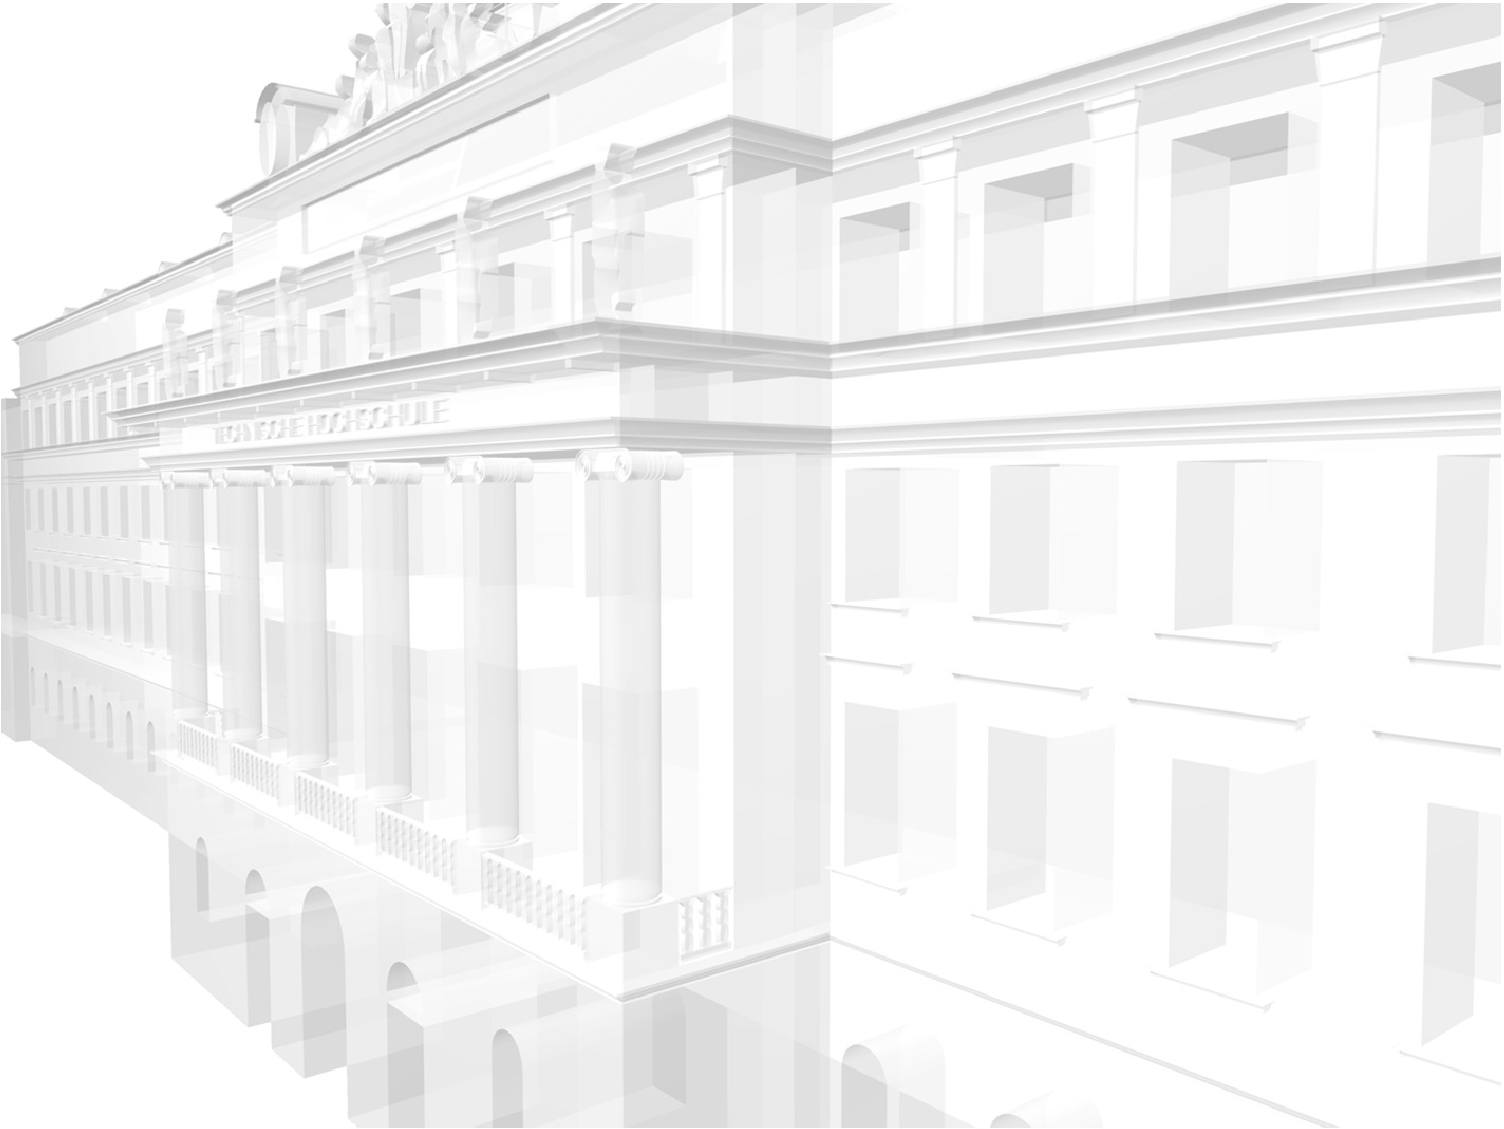
\includegraphics[width=\paperwidth,height=0.5\paperheight]{figures/TU_building.pdf}
}

\title{Towards in-situ nanoscale spatially resolved\hspace{1cm} \\ electron spin resonance in scanning electron microscopes}
\author{\underline{T. Spielauer$^{1}$}, M. Kolb$^{1}$, T. Weigner$^{1}$, A. Pr\"uller$^{1}$, J. Toyfl$^{1}$, G. Boero$^{2}$, P. Haslinger$^{1}$ }
\def\correspondingAuthorEmail{thomas.spielauer@tuwien.ac.at}
\def\website{}
\institute[]{
  {\small
  $^{1}$VCQ, Technische Universität Wien, Atominstitut, Stadionallee 2, 1020 Vienna, Austria; $^{2}$EPFL, BM 3110 Station 17, CH-1015 Lausanne, Switzerland
  }
}


\begin{document}
\begin{frame}[fragile]{}
  \pgfsetfillopacity{0.80}
  \begin{block}{\Large Abstract}
	Electron spin resonance is a widely used analytical tool in medicine, biology
	and material sciences. Traditionally, electron spin systems are driven by microwaves,
	which offers only limited spatial resolution due to the long wavelength of microwaves,
	which can be optimized by sophisticated techniques such as the use of magnetic
	field gradients. We propose a different way of driving spin systems using the
	non-radiative near-field of a modulated electron beam in a scanning electron microscope
	by tuning the microscopes to higher beam currents and using additional beam modulation
	mechanisms. Driving systems with higher harmonics of the modulated beam opens up
	future possibilities to perform in-situ electron spin resonance analysis with high
	spatial resolution down to the nanoscale. To perform our experiments we modified an
	Philips XL30 ESEM to allow for high frequency beam modulation, cryogenic cooling
	of our samples and microwave frequency readout of our spin systems.
  \end{block}
  \begin{columns}[T]
    \begin{column}{.49\linewidth}
%	\begin{block}{\Large The Quantum Klystron}
%        % We call our experiment the \textit{Quantum Klystron}, referencing an established
%        % technology, the Klystron.
%
%        \begin{columns}
%          \begin{column}{0.45\columnwidth}
%          \end{column}
%          \begin{column}{0.55\columnwidth}\begin{center}
%              {\large \textbf{Klystron}}
%            \end{center}
%
%            \begin{itemize}
%              \item Linear beam vacuum tube invented in 1935,\\used as RF and microwave amplifier
%              \item Electron beam velocity modulated by\\microwaves in a (buncher) cavity
%              \item Velocity modulation causes current modulation
%              \item Outcoupling via a catcher cavity
%            \end{itemize}
%          \end{column}
%        \end{columns}
%        \begin{columns}
%          \begin{column}{0.45\columnwidth}
%            % \includegraphics[width=\columnwidth]{figures/zeeman.pdf}
%            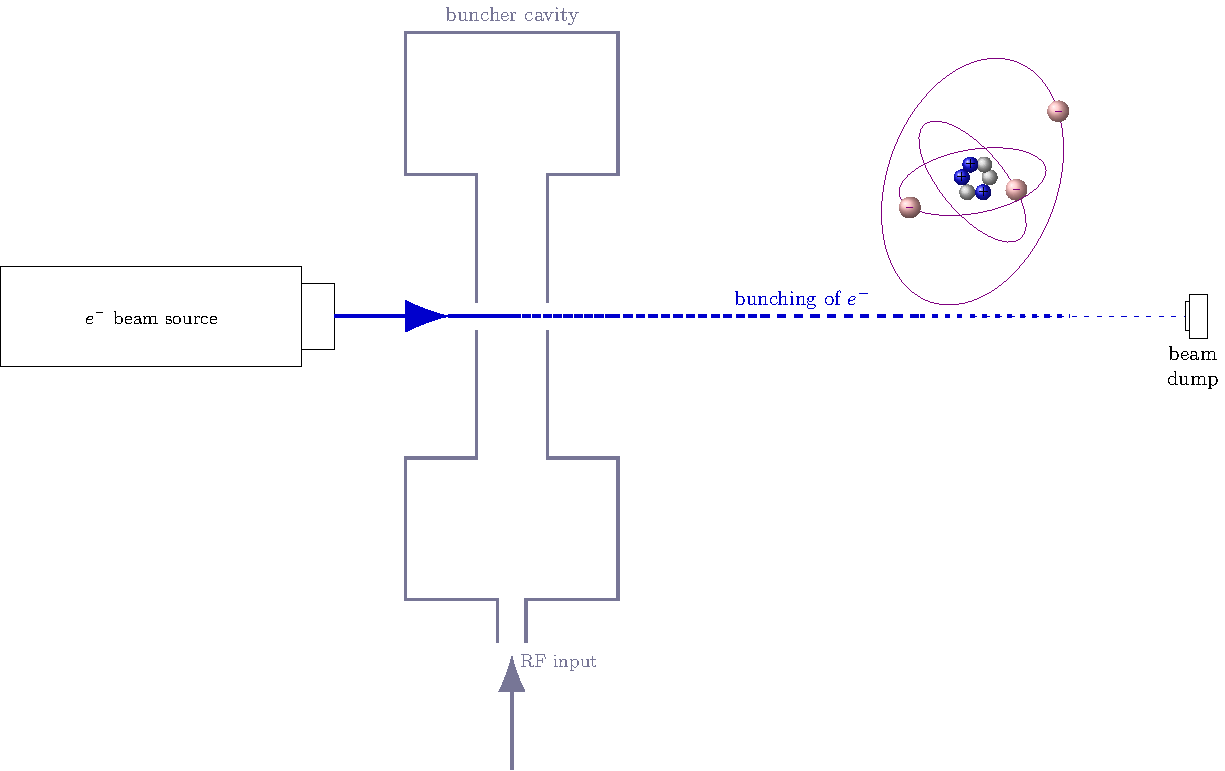
\includegraphics[width=\columnwidth]{figures/qklystron.pdf}
%          \end{column}
%          \begin{column}{0.55\columnwidth}
%            \begin{center}
%              {\large \textbf{Quantum Klystron}}
%            \end{center}
%
%            \begin{itemize}
%              \item Replace catcher cavity by a 2 level\\quantum system (QS)
%              \item Drive the QS using the \textit{non-radiative electro-magnetic near-field}
%                    of the electron beam.
%              \begin{itemize}
%                \item Either modulate in
%                \begin{itemize}
%                    \item \textit{time domain} - bunching / density modulation
%                    \item \textit{spatial domain} - deflection
%                \end{itemize}
%              \end{itemize}
%              \item Paint arbitrary potentials (dipole, quadrupole or multipole transitions)
%              \item High spatial resolution % (electron: $\lambda_{DB}= 27.3 pm$, 202 MHz EM wave: $\lambda=1.48m$)
%            \end{itemize}
%          \end{column}
%        \end{columns}
%      \end{block}
%
%      \begin{block}{\Large Electron Spin Resonance with Modulated Electron Beams}
%        The experiment resembles an electron spin resonance experiment. In contrast to
%        standard electron spin resonance setups where systems are excited using microwaves,
%        we use the \textit{non-radiative electro-magnetic near-field} of an modulated electron beam.
%
%        \begin{columns}
%          \begin{column}{0.3\columnwidth}
%            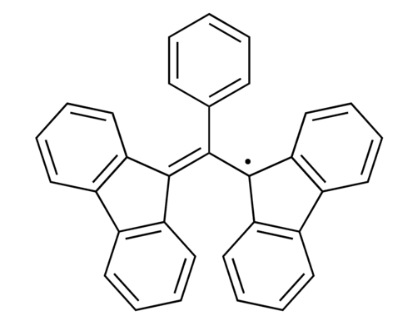
\includegraphics[width=0.67\columnwidth]{figures/bdpa.png}
%          \end{column}
%          \begin{column}{0.3\columnwidth}
%            \includegraphics[width=\columnwidth]{figures/zeeman.pdf}
%          \end{column}
%          \begin{column}{0.4\columnwidth}
%            \includegraphics[width=\columnwidth]{figures/esrsetuppcb.jpg}
%          \end{column}
%        \end{columns}
%
%        \begin{columns}
%          \begin{column}{0.6\columnwidth}
%            \begin{itemize}
%              \item Sample: $C_{33}H_{21}$
%                Koelsch radical ($\alpha,\gamma$-Bisdiphenylene-$\beta$-phenylallyl - BDPA)
%              \item high spin density (1 free spin per 51 atoms)
%              \item Proof of concept experiment at room\\temperature (300K) and liquid nitrogen (77K)
%              % \item Excitation with microwave works at room temperature
%              \item Background subtraction by differential measurement
%            \end{itemize}
%          \end{column}
%          \begin{column}{0.4\columnwidth}
%            \includegraphics[width=\columnwidth]{figures/eprsignal.png}
%          \end{column}
%        \end{columns}
%      \end{block}
%
%      \begin{block}{\Large Temperature Dependence}
%        %We want to move to a cryogenic environment. This is done due to the small signal generated by the modulated electron beam.
%        %
%        The thermal population ratio of spin states depends on temperature:
%        
%        $$\frac{n_2}{n_1} = e^{-\frac{\Delta E}{k_B T}} = \left(e^{- \frac{\Delta E}{k_B}}\right)^\frac{1}{T}$$
%
%        \vskip1ex
%        \begin{columns}
%          \begin{column}{0.5\columnwidth}
%            \includegraphics[width=\columnwidth]{figures/tempn2n1.pdf}
%          \end{column}
%          \begin{column}{0.5\columnwidth}
%            \begin{itemize}
%              \item $300K$ (room temperature): \\ expected $22.9 nV$ signal, $185.83 \sqrt{Hz}^{-1}$ SNR
%              \item $77K$ (liquid nitrogen): \\ expected $89 nV$ signal, $1221.46 \sqrt{Hz}^{-1}$ SNR \\ expected gain $\approx 4$, SNR gain $\approx 7.7$ \\ simple to realize, our choice
%              \item $4K$ (liquid helium): \\ expected $1700 nV$ signal, \\ $103163.45 \sqrt{Hz}^{-1}$ SNR \\ expected gain $\approx 75$, \\ SNR gain $\approx 649.5$
%            \end{itemize}
%          \end{column}
%        \end{columns}
%        \vskip1ex
%
%        % Either remove or simpler (only for Poissonian noise)
%        Averaging increases the effective SNR by $\sqrt{N}$ for $N$ iterations. \textit{Doubling SNR}
%        of a single run decreases the number of required averages by a factor of four. A gain
%        of 4 decreases measurement time by a factor of 16, a gain of 650 would decrease
%        measurement time by about half a million.
%
%        \begin{columns}
%          \begin{column}{0.65\columnwidth}
%            \begin{itemize}
%              \item Initial tests by cooling BDPA sample in liquid nitrogen bath
%              \item Scanned $B_0$ field, excited with microwaves (no electron beam)
%              \item Compared amplitudes at 300K and 77K
%              \item Resonance frequency of impedance match drifts
%              \item Signal gain $\approx 4$
%            \end{itemize}
%          \end{column}
%          \begin{column}{0.35\columnwidth}
%            \includegraphics[width=\columnwidth]{figures/signals300_77.pdf}
%          \end{column}
%        \end{columns}
%      \end{block}

%%      \begin{block}{\Large Contact}
%%          Thomas Spielauer \\ 
%%          Technische Universität Wien, Atominstitut \\ 
%%          thomas.spielauer@tuwien.ac.at
%%      \end{block}
    \end{column}

    % -------------------------------------------------------------

    \begin{column}{.49\linewidth}
%      \begin{block}{\Large Experimental Setup}
%        \begin{columns}
%          \begin{column}{0.4\columnwidth}
%            \includegraphics[width=\columnwidth]{figures/cryoquak02.png}
%          \end{column}
%          \begin{column}{0.6\columnwidth}
%              \begin{itemize}
%                \item Barium-Strontium cathode, electrostatic beam deflection. Current $\geq 10 \mu A$ at
%                    up to $2.2 kV$.
%                \item Modulation frequency $\approx 250 MHz$
%                \item Two cameras imaging phosphor screens
%                \item Cooling with liquid nitrogen
%                \item Vacuum $\leq 10^{-8}$ mbar
%              \end{itemize}
%          \end{column}
%        \end{columns}
%      \end{block}
%
%      \begin{block}{\Large Readout and Radio Frequency Setup}
%        \begin{columns}
%          \begin{column}{0.6\columnwidth}
%            \begin{itemize}
%              \item Inductive readout by a microcoil on a printed circuit
%                board (also including impedance match)
%              % \item Printed circuit board with two coils and impedance match
%              \item Second microcoil for reference measurements
%              \item BDPA inside microcoil (2 windings, $2.58mm$ x $1.14mm$
%                    outer diameter, $1.5mm$ x $0.5mm$ sample area) in milled pocket
%            \end{itemize}
%          \end{column}
%          \begin{column}{0.4\columnwidth}
%            %\includegraphics[width=\columnwidth, angle=180]{figures/pcb01.jpg}
%
%            %\includegraphics[width=\columnwidth]{figures/pcb02.jpg}
%            \includegraphics[width=\columnwidth]{figures/microcoilpcb.png}
%          \end{column}
%        \end{columns}
%
%        \begin{columns}
%          \begin{column}{0.6\columnwidth}
%            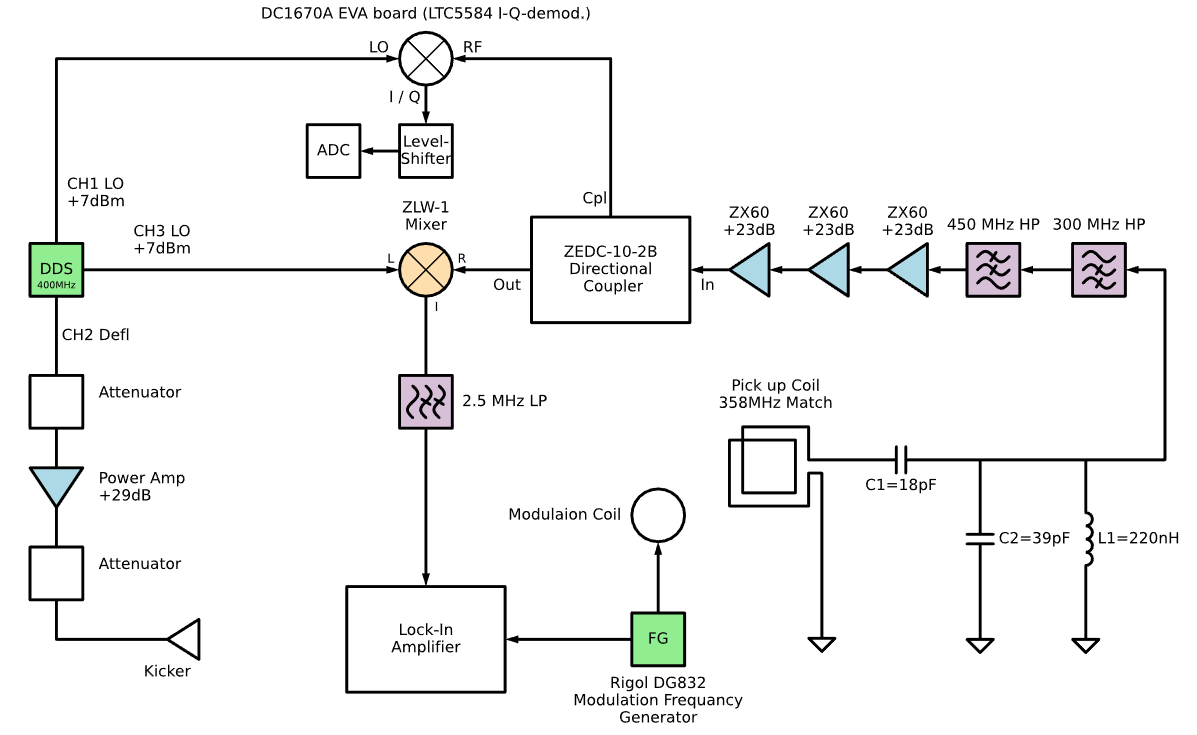
\includegraphics[width=\columnwidth]{figures/rfsetup.png}
%          \end{column}
%          \begin{column}{0.4\columnwidth}
%            \begin{itemize}
%              \item Two independent channels of an AD9959 based DDS
%              \item Applying $5.123 kHz$ modulation field $B_m$ parallel to $B_0$
%                for lock-in detection
%            \end{itemize}
%          \end{column}
%        \end{columns}
%      \end{block}
%  
%      \begin{block}{\Large First Runs at Room Temperature}
%        \begin{columns}
%          \begin{column}{0.4\columnwidth}
%            \begin{itemize}
%                \item Electron beam at $2.2 kV$
%                \item Deflected at $202 MHz$
%                \item Scanning distance to microcoil (\textit{slow position})
%                \item Beam wiggled by $B_m$ field
%                \item Coupling of \textit{near-field} into microcoil
%                \item Shows $\frac{1}{r}$ behaviour (Biot-Savart law)
%            \end{itemize}
%          \end{column}
%          \begin{column}{0.6\columnwidth}
%            \includegraphics[width=\columnwidth]{figures/beamcoupling.pdf}
%          \end{column}
%        \end{columns}
%      \end{block}
%
%%      \begin{block}{\Large First runs on conventional test setup}
%%        We did some initial tests on our setup by simply cooling a PCB containing our
%%        BDPA sample in a liquid nitrogen bath.
%%
%%        \begin{columns}
%%          \begin{column}{0.4\columnwidth}
%%            \begin{itemize}
%%              \item Excited using microwaves via directional coupler
%%              \item Scanned $B_0$ field
%%              \item Compared amplitudes at room temperature and $77K$
%%              \item Resonance frequency of match
%%              \item Signal gain $\approx 4$
%%            \end{itemize}
%%          \end{column}
%%          \begin{column}{0.6\columnwidth}
%%            % \includegraphics[width=\columnwidth]{figures/cryoamplitudes.pdf}
%%            \includegraphics[width=\columnwidth]{figures/signals300_77.pdf}
%%          \end{column}
%%%        \end{columns}
%%
%%        We saw the expected increase in signal amplitude as well as a shift of our
%%        impedance match that we have to compensate for.
%%      \end{block}
%
      \begin{block}{\Large References \& Acknowledgements}
        [1] D. Rätzel, D. Hartley, O. Schwartz, P. Haslinger, A Quantum
        Klystron - Controlling Quantum Systems with Modulated Electron Beams.
        \textit{Phys. Rev. Research 3, 023247 (2021)}
      \end{block}

      \begin{block}{}
        \begin{columns}
          \begin{column}{0.3\columnwidth}
            
\includegraphics[width=\columnwidth]{figures/logo-fwf.png}
          \end{column}
          \begin{column}{0.2\columnwidth}
            
\includegraphics[width=\columnwidth]{figures/logo-ffg.png}
          \end{column}
          \begin{column}{0.4\columnwidth}
            
\includegraphics[width=\columnwidth]{figures/logo-oeaw.png}
          \end{column}
          \begin{column}{0.07\columnwidth}
            
\includegraphics[width=\columnwidth]{figures/logo-start.png}
          \end{column}
        \end{columns}
      \end{block}


      \begin{block}{\Large Join our Team!}
        {\Large We have open positions for Master, PhD and PostDoc!}

        Visit us at \texttt{http://www.haslingerlab.com/}, E-Mail: \texttt{philipp.haslinger@tuwien.ac.at}
      \end{block}
    \end{column}

  \end{columns}

\end{frame}
\end{document}
